\documentclass[a4paper, 12pt]{article}
\usepackage[utf8]{inputenc}
\usepackage[warn]{mathtext}
\usepackage[russian]{babel}
\usepackage[T2]{fontenc}
\usepackage[warn]{mathtext}
\usepackage{caption}

\usepackage{graphicx}
\graphicspath{ {images/} }
\usepackage{tikz}
\usepackage{pgfplots}

\usepackage{amsmath}
\usepackage{floatflt}
\usepackage[left=20mm, top=20mm, right=20mm, bottom=20mm, footskip=10mm]{geometry}

\usepackage{multicol}
\setlength{\columnsep}{2cm}

\usepackage{multicol}
\setlength{\columnsep}{2cm}
\usepackage{hyperref}

\begin{document}
	
\begin{titlepage}
	\centering
	\vspace{5cm}
	{\scshape\LARGE Московский физико-технический институт \par}
	\vspace{4cm}
	{\scshape\Large Лабораторная работа 4.6.1 \par}
	\vspace{1cm}
	{\huge\bfseries Интерференция электромагнитных волн миллиметрового диапазона \par}
	\vspace{1cm}
	\vfill
\begin{flushright}
	{\large выполнил студент 924 группы ФОПФ}\par
	\vspace{0.3cm}
	{\LARGE Панферов Андрей}
\end{flushright}
	

	\vfill

% Bottom of the page
	Долгопрудный, 2021 г.
\end{titlepage}

\paragraph*{Цель работы:} изучение интерференции электромагнитных волн миллиметрового диапазона с применением двух оптических интерференционных схем, экспериментальное определение длины волны излучения и показателя преломления диэлектрика.
\paragraph*{В работе используются:} приёмно-передающая система радиоволн миллиметрового диапазона; металлические зеркала; микрометрический винт; проволочная решётка; пластина из диэлектрика.
$$$$
Если в некоторой точке пространства происходит суперпозиция двух когерентных одинаково поляризованных волн с интенсивностями $I_1$ и $I_2$ и с разностью фаз $k\Delta$, то интенсивность $I$ результирующего колебания определяется соотношением
$$I = I_1 + I_2 + 2\sqrt{I_1 I_2} \cdot \cos{k\Delta}$$
Интенсивность максимальна при 
$$k\Delta = 2m\pi$$
и минимальна при
$$k\Delta = \left(2m + 1\right)\pi$$
\paragraph*{Экспериментальная установка:} Источником радиоволн в работе является высокочастотный генератор Г4–115 на трёх отражательных клистронах, перекрывающих вместе полосу частот от 25,80 ГГц до 37,50 ГГц, разделённую на три поддиапазона, соответствующие отдельным клистронам. Генерирующий при выбранной настройке клистрон возбуждает в прямоугольном металлическом волноводе сечением 7,2×3,4 мм2 электромагнитную волну, которая распространяется вдоль волновода и с помощью рупорной антенны излучается в пространство. Задача антенны заключается в том, чтобы сделать излучение более направленным.

\begin{figure}[h]
    \centering
    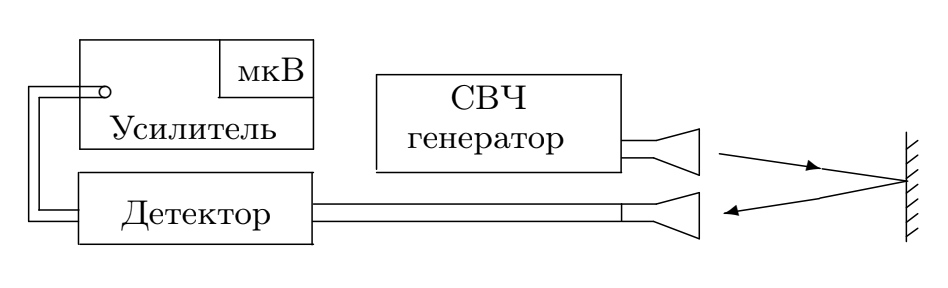
\includegraphics[width=15cm]{reflection.png}
    \caption{Приёмно-передающая система СВЧ-диапазона}
    \label{fig:reflection}
\end{figure}

Отражённое от препятствия электромагнитное излучение, попадая в рупорную антенну приёмника, распространяется по волноводу, в котором имеется детектор высокочастотных колебаний, работающий в квадратичном режиме. Поэтому ток детектора пропорционален интенсивности $I$ волны, попадающей в приёмную антенну. Сигнал с выхода детектора усиливается и измеряется микровольтметром. Принципиальная схема приёмно-передающего тракта представлена на рис. \ref{fig:reflection}.

\newpage

\section*{Ход работы}

\paragraph*{Проверка закона Малюса}

Применяемый в настоящей работе передатчик излучает линейно поляризованную волну, электрический вектор \textbf{E} которой перпендикулярен широкой стенке волновода. Приёмник также может принимать только линейно поляризованную волну. Для установления связи в системе, изображённой на рис. \ref{fig:reflection}, необходимо, чтобы широкие стенки волноводов передатчика и приёмника были параллельны друг другу.

Если одну из антенн повернуть относительно луча на некоторый угол $\alpha$, то интенсивность принимаемого сигнала будет изменяться по закону

$$I = I_0 \cdot \cos^2(\alpha)$$

Выполнение на опыте этого закона свидетельствует о том, что передатчик излучает, а приёмная система принимает линейно поляризованную волну.

\begin{enumerate}
    \item На дальнем от генератора конце стола закрепим зеркало. Зеркально от излучателя расположим приемник сигнала. Подстроим сигнал, передвигая приёмную антенну и слегка поворачивая её вокруг горизонтальной оси. Методом последовательных приближений ещё раз отрегулируем положение зеркала и антенн, чтобы настроиться на максимум сигнала.
    \item Снимем зависимость уровня сигнала $I$ от угла поворота $\alpha$ приёмной антенны относительно луча. Результаты занесем в Таблицу \ref{table:angle}. Построим график соответствующей зависимости.
    
    \begin{minipage}{0.4\textwidth}
        \begin{tabular}{|l|l|l|}
        \hline
        $I$, мкВ & $\alpha$, $\deg$ & $\cos^2\left(\alpha\right)$ \\ \hline
        75       & 0        & 1                          \\ \hline
        65       & 23       & 0.85                       \\ \hline
        55       & 31       & 0.73                       \\ \hline
        45       & 39       & 0.60                       \\ \hline
        35       & 48       & 0.45                       \\ \hline
        25       & 54       & 0.35                       \\ \hline
        21       & 63       & 0.21                       \\ \hline
        \end{tabular}
        \captionof{table}{Зависимость интенсивности от угла}
        \label{table:angle}
    \end{minipage}
    \begin{minipage}{0.6\textwidth}
        \begin{center}
            \begin{tikzpicture}[scale=1]
                \begin{axis}[
                    	axis lines = middle,
                    	xlabel = {$\cos^2\left(\alpha\right)$},
                        ylabel = {$I$, мкВ},
                    	ylabel style={red, scale=1},
                        xlabel style={red, scale=1},
                    	title={Зависимость интенсивности от угла},
                    	table/col sep=semicolon,
                    ]
            	    \addplot +[blue, only marks]  plot[error bars/.cd, x dir=both, x explicit] coordinates{(1, 75) +- (0, 0) (0.85, 65) +- (0.01, 0.01) (0.73, 55) +- (0.015, 0.015) (0.60, 45) +- (0.017, 0.017) (0.45, 35) +- (0.017, 0.017) (0.35, 25) +- (0.017, 0.017) (0.21, 21) +- (0.014, 0.014)};
        		    \addplot[color=red, domain=0:1]{75 * x};
            	\end{axis}
            \end{tikzpicture}
        \end{center}
    \end{minipage}
\end{enumerate}
    
    Как видно из графика, закон Малюса действительно выполняется.
    
\paragraph*{Интерференция волн, отражённых от зеркала и решётки}

\begin{enumerate}
    \item Закрепим на фиксаторах перед зеркалом металлическую решётку и снимем зависимость интенсивности $I$ от координаты $x$ подвижного зеркала, занесем результаты в Таблицу \ref{table:inter}. Построим График \ref{} зависимости $I(x)$, определим по графику частоту излучения $\lambda$ и сравним с частотой генератора.
    
    \begin{minipage}{0.45\textwidth}
    \begin{center}
        \begin{tabular}{|l|l|l|l|}
        \hline
        $x$, мм & $I$, мкВ & $x$, мм & $I$, мкВ \\ \hline
        0       & 16       & 3.5     & 30       \\ \hline
        0.25    & 15       & 3.75    & 24       \\ \hline
        0.5     & 12       & 4       & 20       \\ \hline
        0.75    & 10       & 4.25    & 14       \\ \hline
        1       & 9        & 4.5     & 12       \\ \hline
        1.25    & 8        & 4.75    & 11       \\ \hline
        1.5     & 5        & 5       & 10       \\ \hline
        1.75    & 2        & 5.25    & 9        \\ \hline
        2       & 2        & 5.5     & 7        \\ \hline
        2.25    & 16       & 5.75    & 4        \\ \hline
        2.5     & 16       & 6       & 3        \\ \hline
        2.75    & 24       & 6.25    & 3        \\ \hline
        3       & 27       & 6.5     & 10       \\ \hline
        3.25    & 28       & 6.75    & 19       \\ \hline
                &          & 7       & 25       \\ \hline
        \end{tabular}
        \captionof{table}{Интерференция на зеркале с решеткой}
        \label{table:inter}
    \end{center}
    \end{minipage}
    \begin{minipage}{0.55\textwidth}
    \begin{center}
            \begin{tikzpicture}[scale=1]
                \begin{axis}[
                    	axis lines = middle,
                    	xlabel = {$x$, мм},
                        ylabel = {$I$, мкВ},
                    	ylabel style={red, scale=1},
                        xlabel style={red, scale=1},
                    	title={Интерференция на зеркале с решеткой},
                    	table/col sep=semicolon,
                    ]
            	    \addplot +[blue, only marks] table[x=x, y=I]{HZ.csv};
        		    \addplot[color=red, domain=0:7]{0};
            	\end{axis}
            \end{tikzpicture}
        \end{center}
    \end{minipage}
\end{enumerate}

По графику найдем длину волны 
$$\lambda = 8.6 \pm 0.4 \text{мм}$$
И, соответственно, частоту 
$$f = 35 \pm 2 ГГц$$

    \paragraph*{Интерферометр Майкельсона}
    
    \begin{enumerate}
        \item $$\:$$
        \begin{minipage}{0.5\textwidth}
            Измерим позицию $n$-того максимума от координаты, занесем результаты в Таблицу \ref{table:maximums}, и по ней найдем длину волны излучения:
            $$\lambda = 8.250 \pm 0.002 \text{ мм}$$
            И соответственно частоту
            $$f = 36.12 \pm 0.001 \text{ ГГц}$$
        \end{minipage}
        \begin{minipage}{0.5\textwidth}
        \begin{center}
            \begin{tabular}{|l|l|}
            \hline
            n & $x$, мм \\ \hline
            0 & 0       \\ \hline
            1 & 4.10    \\ \hline
            2 & 8.12    \\ \hline
            3 & 12.22   \\ \hline
            4 & 16.33   \\ \hline
            5 & 20.54   \\ \hline
            6 & 24.75   \\ \hline
            \end{tabular}
            \captionof{table}{Координаты максимумов}
            \label{table:maximums}
        \end{center}
        \end{minipage}
        
    \item Измерим интенсивности в плечах интерферометра $I_1 = 10$ мкВ, $I_2 = 11$ мкВ. Тщательно промерим один период интерференции. Занесем результаты в таблицу \ref{table:peak} 
    
    \begin{minipage}{0.5\textwidth}
    \begin{center}
            \begin{tikzpicture}[scale=1]
                \begin{axis}[
                    	axis lines = middle,
                    	xlabel = {$x$, мм},
                        ylabel = {$I$, мкВ},
                    	ylabel style={red, scale=1},
                        xlabel style={red, scale=1},
                    	title={Один пик интерференции},
                    	table/col sep=semicolon,
                    ]
            	    \addplot +[blue, only marks]       table[x=x, y=I]{Fabri.csv};
            	    \addplot[color=red, domain=0:5]{21 + 21 * cos(360 * x / 4.125 - 87)};
            	\end{axis}
            	\label{graph:Fabri}
            \end{tikzpicture}
        \end{center}
    \end{minipage}
    \begin{minipage}{0.5\textwidth}
    \begin{center}
        \begin{tabular}{|l|l|l|l|}
        \hline
        $x$,  мм & $I$, мкВ & $x$,  мм & $I$, мкВ \\ \hline
        0        & 42       & 2.5      & 5        \\ \hline
        0.25     & 40       & 2.75     & 0        \\ \hline
        0.5      & 41       & 3        & 0        \\ \hline
        0.75     & 40       & 3.25     & 0        \\ \hline
        1        & 40       & 3.5      & 4        \\ \hline
        1.25     & 41       & 3.75     & 10       \\ \hline
        1.5      & 36       & 4        & 14       \\ \hline
        1.75     & 31       & 4.25     & 21       \\ \hline
        2        & 23       & 4.5      & 27       \\ \hline
        2.25     & 15       & 4.75     & 33       \\ \hline
                 &          & 5        & 39       \\ \hline
        \end{tabular}
        \captionof{table}{Интерференция}
        \label{table:peak}
    \end{center}
    \end{minipage}
    Построим График \ref{graph:Fabri} соответствующей зависимости. Нанесем на него теоретическую зависимость.
    
    \item Поставим в пазы подвижного зеркала тонкую пластину толщины $d = 3.2$ мм из тефлона и, изменяя его положение, определим величину $\delta x$ — смещение интерференционного максимума от прежнего положения.
    $$\delta x \approx 1 \text{ мм} \implies n = 1 + \frac{\delta x}{d} \approx 1.33$$
    \end{enumerate}
    
    \section*{Вывод}
    \begin{itemize}
        \item Мы проверили закон Малюса (и убедились в его справедливости)
        \item Мы пронаблюдали и измерили интерференцию волн в плоской пластине и получили значение длины волны $f_1 = 35 \pm 2 \text{ ГГц}$
        \item Мы собрали и измерили интерферометр Майкельсона, точно получив длину волны и, соответственно, частоту $f_2 = 36.12 \pm 0.001 \text{ ГГц}$
        \item Сравним две частоты выше с частотой, на которую был настроен излучатель: $f_{emitter} = 36.25$ ГГц
        \item Мы измерили показатель преломления тефлона $n = 1.33 \pm 0.02$ ($n_{tabl} = 1.4$)
        
        
    \end{itemize}
    
\end{document}